\PassOptionsToPackage{table, dvipsnames}{xcolor}
\documentclass[11pt]{beamer} %%

%%% option passed to the outer theme
% fixedCircCnt,   % (moving is deault)
\usetheme[progressstyle= movingCircCnt]{Feather}


%%xcolor=dvipsnames,
%-------------------------------------------------------
% INCLUDE PACKAGES
%-------------------------------------------------------

\usepackage[utf8]{inputenc} 
\usepackage{graphicx}
\usepackage{tikz}
\usetikzlibrary{decorations.fractals}
\usepackage{wrapfig}
\usepackage[english]{babel}
\usepackage{amsmath}
\usepackage{braket}
\usepackage{wrapfig}
\usepackage{mathpazo} 
\usepackage{amssymb}
\usepackage{amsmath}
\usepackage{amsfonts}
%\usepackage{mathrsfs}
\usepackage{slashed} % Dirac slash
\usepackage{pifont}

%%%% multimedia
%%\usepackage{multimedia}
%%\usepackage{hyperref}


%%%% fonts
\usepackage{tgtermes}
%% change font of the document 
%\renewcommand*{\familydefault }{\mrdefault}
\usefonttheme{professionalfonts} % using non standard fonts for beamer
\usefonttheme{serif} % default family is serif
\usepackage{fontspec}
\setmainfont{Latin Modern Roman}

%%%% colors
% Change the frame title text color:
\setbeamercolor{frametitle}{fg=BurntOrange}
% Change the normal text color background:
\setbeamercolor{normal text}{fg=black,bg=white}
%%% color equations 
\usepackage[skins,theorems]{tcolorbox}
\tcbset{highlight math style={enhanced,
  colframe=red,colback=white,arc=0pt,boxrule=1pt}}

%%%% colourful equation box
\tcbset{highlight math style={enhanced,
  colframe=red,colback=white,arc=0pt,boxrule=1pt}}
\newcommand{\eqbox}[3]
           {
             \tcbhighmath[boxrule=2pt,arc=1pt,colback=#1!10!white,colframe=#2!40,
               drop fuzzy shadow=white] {#3}
           }

%%%%  tables
%%\usepackage[landscape]{geometry}
\usepackage{multirow}
\usepackage{changepage}
\usepackage{longtable}
\usepackage{booktabs}

%% for pdf input
\usepackage{pdfpages}

\usepackage{forloop}

%%%% set footers
\setbeamertemplate{footline}[text line]{%
  \parbox{0.6\linewidth}{\vspace*{-5pt}\hspace*{1.0cm}
    \textcolor{BurntOrange}{--- Particle Detectors}}\hfill
  \parbox{0.4\linewidth}{\vspace*{-5pt}\hspace*{2.5cm}
    \textcolor{BurntOrange}{  Fall 2017 ---}}\hfill
}
%%\setbeamertemplate{footline}[page number]

% colored hyperlinks
\newcommand{\chref}[2]
           {
             \href{#1}{{\usebeamercolor[bg]{Feather}#2}}
           }

%%%% few extra commands
\renewcommand{\(}{\begin{columns}}
\renewcommand{\)}{\end{columns}}
\newcommand{\<}[1]{\begin{column}{#1}}
\renewcommand{\>}{\end{column}}

\newcommand{\itt}{\begin{itemize}}
\newcommand{\tti}{\end{itemize}}

\newcommand{\img}[1]{\includegraphics[width=\linewidth]{./Images/#1}}

\newcommand{\hlt}[2]{\textcolor{#1}{\textbf{#2}}}
\newcommand{\ntit}[1]{\qquad\qquad\qquad\qquad\hlt{blue}{\Large #1}\\~\\}
%% \newcommand{\hlt1}[1]{\textcolor{Goldenrod}{\textbf{#1}}}
\newcommand{\cmark}{\ding{51}}%
\newcommand{\done}
           {
             \rlap{$\square$}
                  {\raisebox{2pt}
                    {
                      \large\hspace{0.1pt}
                      \textcolor{green}{\cmark}
                    }
                  }
                  \hspace{-2.5pt}
           }

           
%%% counting backup slides
\newcommand{\beginbackup}
           {
             \newcounter{framenumbervorappendix}
             \setcounter{framenumbervorappendix}{\value{framenumber}}
           }
\newcommand{\backupend}
           {
             \addtocounter{framenumbervorappendix}{-\value{framenumber}}
             \addtocounter{framenumber}{\value{framenumbervorappendix}} 
           }

%%%% Loading packages DONE!
\logo{
\includegraphics[scale = 0.2]{./Images/SFU_logo.jpg}}

\begin{document}
%%%% SLIDE 1: title page
\begin{frame}
	\vspace{0.9cm}

\title[]{Cherenkov and Transition-Radiation Detectors}
\author{Sina Bahrasemani\\
  \vspace{0.2in}
}
\date{
  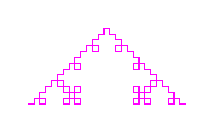
\begin{tikzpicture}[decoration=Koch curve type 1] 
    \draw[Magenta] decorate{ decorate{ decorate{ (0,0) -- (2,0) }}}; 
  \end{tikzpicture}  
  \\
  \vspace{0.2cm}
  \today
}
\titlepage
\end{frame}

%%%% SLIDE 2: outline page
% \begin{frame}{Outline}
% \small
% \tableofcontents
% \end{frame}

%%%% SLIDE 3: introduction
\section{Introduction} 
\begin{frame}{\textcolor{Goldenrod}{Introduction}}
  \begin{center}
  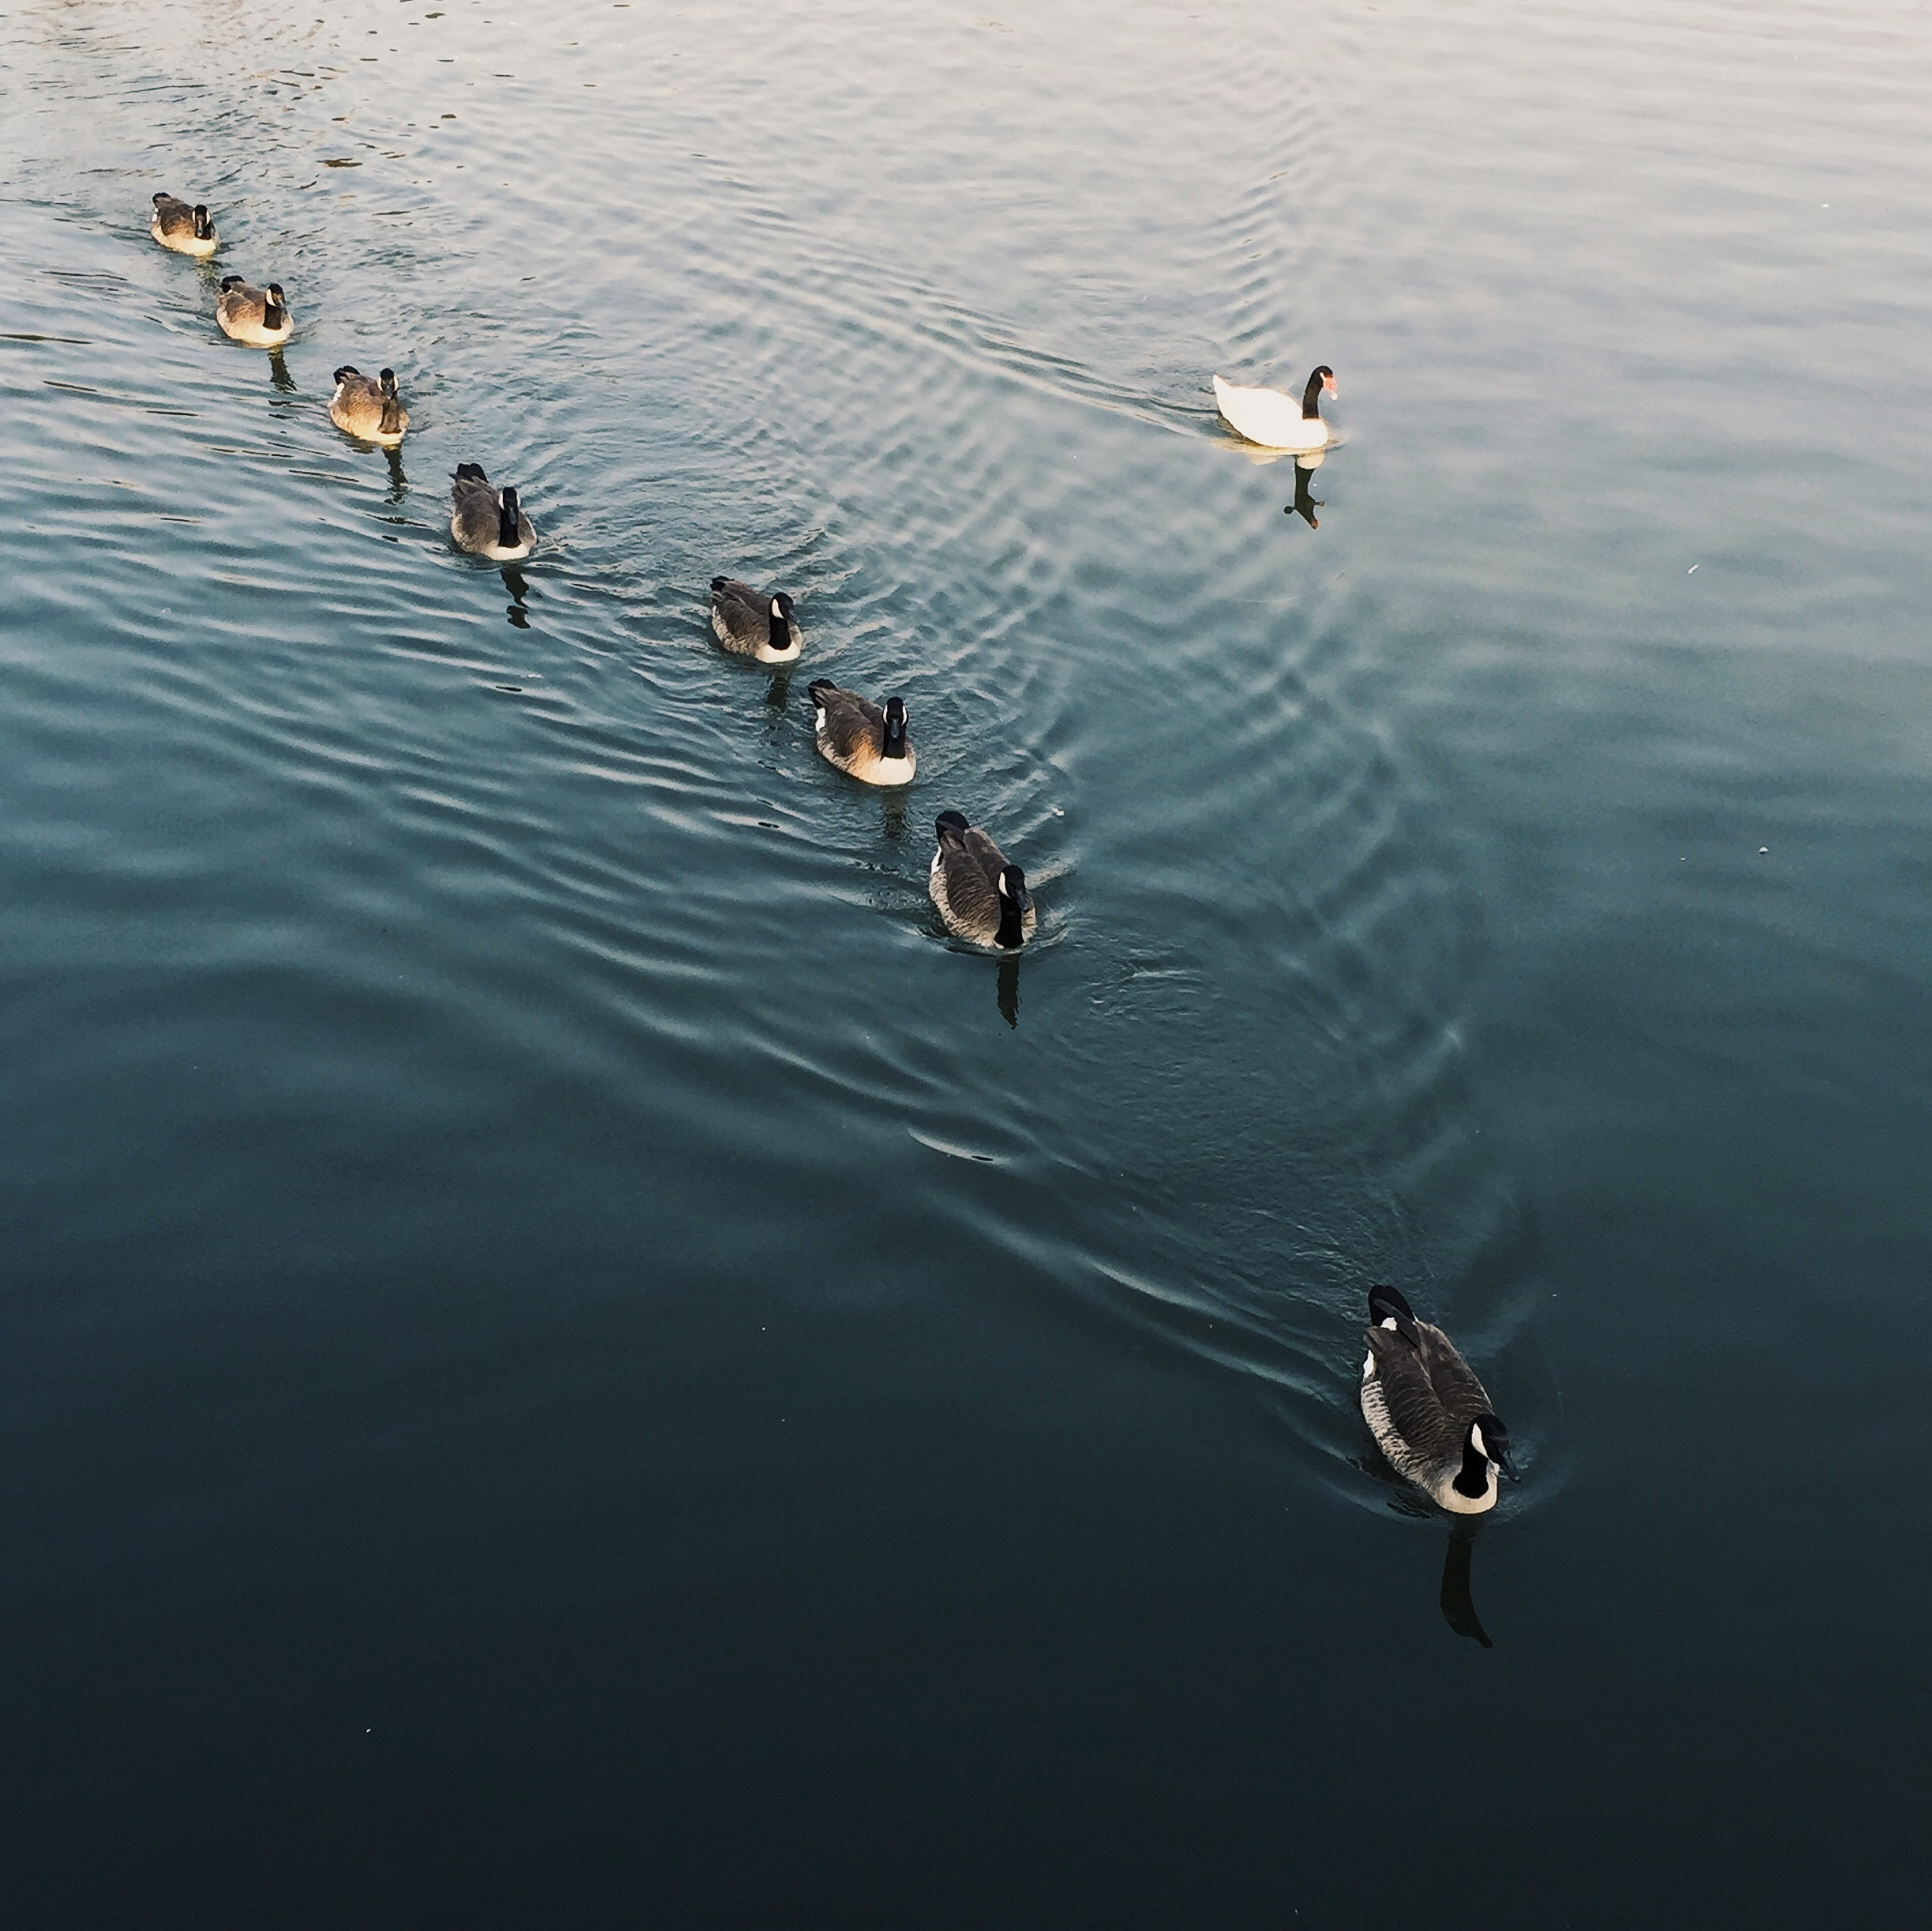
\includegraphics[width=0.6\textwidth,
  height=0.4\textheight]{./Images/little_duck_swim}\\
  \end{center}
  \itt
  \item[$\bullet$] What happens to cocenteric water waves, if duck
    (wave source) moves ?
    \itt
  \item \hlt{Magenta}{If the duck moves faster than the waves generated by itself,
    then the waves can not propagate forward from the duck, instead
    forming a shock front.}
    \tti
  \tti
\end{frame}

%% cite An Introduction to Cherenkov Radiation, Hadiseh	Alaeian
%%%% SLIDE 4
\subsection{Cherenkov Radiation}
\begin{frame}{\textcolor{Goldenrod}{Cherenkov Radiation}}
  \(
  \<{0.35\textwidth}
  \img{cherenkov_rad}
  \>
  \<{0.75\textwidth}
  \hlt{LimeGreen}{The Cherenkov radiation is analogous with the shock
    waves from a duck swimming in a pond}
  \itt
\item When a charged particle moves
  inside a medium it excites the atoms and molecules of the
  matter and they emit radiation.
\item According to the Huygens principle, the emitted waves move out
  spherically at the phase velocity of the medium.
\item \hlt{Magenta}{This radiation depends on the speed of charged particle and the
    properties of the matter}
  \tti
  \>
  \)
\end{frame}

%%%% SLIDE 5
\begin{frame}{\textcolor{Goldenrod}{Cherenkov Radiation}}

\itt  
\item[$\Box$] If the particle motion is slow, the radiated waves bunch
  up slightly in the direction of motion, but they do not cross.
\item[$\Box$] \hlt{Magenta}{However if the particle moves faster than the light
    speed, the emitted waves add up constructively leading to a coherent
  radiation at angle $\theta$ with respect to the particle direction,
  known as Cherenkov radiation.}
\item[$\Box$] \hlt{Red}{The signature of the effect is a cone of
    emission in the direction of particle motion}
\tti
\end{frame}


\begin{frame}{\textcolor{Goldenrod}{Cherenkov $\theta_C$}}
  \hlt{NavyBlue}{For a particle with momentum $p_{\mu}$,  
    moving in a medium with refractive index $n$.
    If the radiated photon makes angle $\theta$ with the direction
    of propagation, then conservation of 4-momentum requires that:}
  \[
    \begin{aligned}
      &\vec{P}^2_i = \vec{P}^{2}_{f} + \vec{P}^2_{\gamma} -2P_f P_{\gamma}
      \cos{\theta_{p, \gamma}}\\
      & E_i = E_f + E_{\gamma} \to \sqrt{P^2_i c^2 + m^2_0 c^4} =
      \sqrt{P^2_f c^2 + m^2_0 c^4} + h\nu\\
      & \alert{\cos{\theta_{p, \gamma}} = \frac{1}{n \beta } + 
        \frac{(n^2 -1)h\nu}{2P_i c n}}
    \end{aligned}
    %% \quad\nu = \frac{c}{n \lambda}}
    %% \frac{1}{\beta c}= \frac{2\sqrt{P^2_i c^2 + m^2_0 c^4}}{2P_i c}
  \]
\end{frame}

\begin{frame}{\textcolor{Goldenrod}{Cherenkov Radiation:
      Characteristics}}
  \itt
\item[$\Box$] \hlt{Red}{There's no emission below a threshold velocity
    $\beta_t = \frac{1}{n}$}.
\item[$\Box$] \hlt{LimeGreen}{For relativistic particles, the
    Cherenkov radiation occurs at a fixed angle.}
\item[$\Box$] For non-relativistic particles There the radiation is
  mainly caused by the different polarization dipoles of the medium in
  front and back of the moving particle.
\item[$\Box$] \hlt{Magenta}{For dispersive mediums (refractive index
    varies with frequency) $\to$ the photons of different energy are
    scattered in various angles.}
\item[$\Box$] if the refractive index of a materials drops below 1, no
  Cherenkov radiation can be observed within that range.
  \tti
\end{frame}
\begin{frame}{\textcolor{Goldenrod}{Cherenkov Radiation}}
  %% cite :http://www.ikp.uni-koeln.de/groups/reiter/lehre/files/det2014/det21Cher.pdf
  \begin{center}
    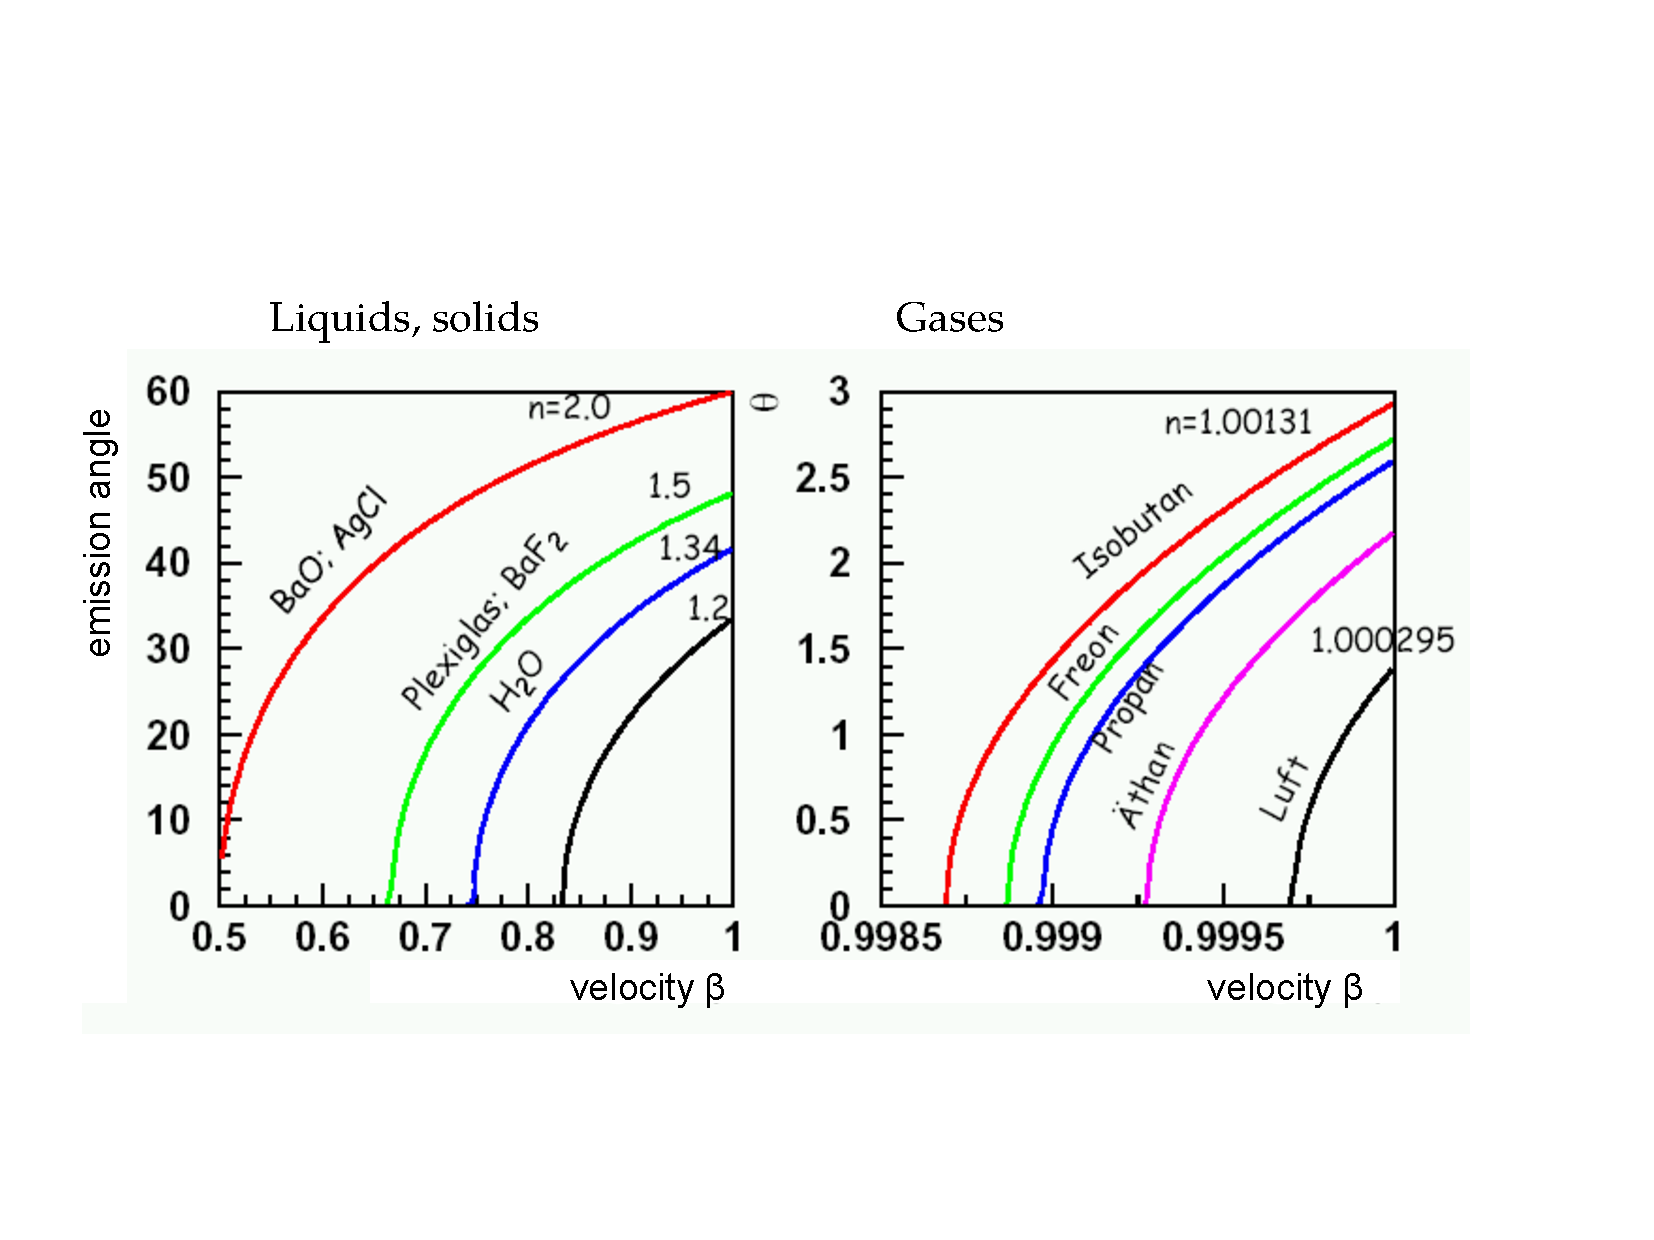
\includegraphics[width=0.7\textwidth, height=0.4\textheight]{./Images/cherenkov_angle_vs_beta}
  \end{center}
  \itt
\item small $n$ is good for relativistic particles $\to$ small
  emission angle
\item large $n \to $ large emission angle.
  \tti
\end{frame}

\begin{frame}{\textcolor{Goldenrod}{Cherenkov Radiation Spectrum}}
 \hlt{Blue}{The number of radiation emitted $dE$ per unit length $dx$ per unit
 frequency $d\omega $ is  given by the Frank-Tamm formula:}
 %% \url{http://www.thphys.uni-heidelberg.de/~wolschin/eds14_3s.pdf}
 %% cite : Bolotovskii, Frenkel: „I. Tamm Selected Papers“
 %% Tamm, Frank: „Coherent Visible Radiation of fast Electrons Passing  rough Ma er“
 \[
   \frac{dE}{dx d\lambda} =  \frac{4\pi Z^2 r_e mc^2}{\lambda^3}[ 1 -
   \frac{1}{n^2\beta^2}] 
 \]
 \itt
\item $r_e$ is classical electron's radius
\item \textcolor{blue}{The emitted energy is peaked at short wavelengths(blue light)}
  \tti
\end{frame}


\begin{frame}{\textcolor{Goldenrod}{Cherenkov Radiation Spectrum}}
  In terms of emitted number of photos per unit length per unit
  wavelength:
  \[
    \frac{dN}{dx d\lambda} =  \frac{2\pi \alpha}{\lambda^2}[ 1 -
    \frac{1}{n^2\beta^2}] ; \quad \alpha = 1/137
  \]
  If $n(\lambda) \approx const.$ over some range ($\lambda_i \to \lambda_f$), then using ($\cos\theta =
  1/n\beta$)
  \[
    \begin{aligned}
      &\textcolor{Magenta}{\frac{dE}{dx} = 2 \pi^2 r_e mc^2 \sin^2\theta
      [\frac{1}{\lambda^2_i} - \frac{1}{\lambda^2_f}]}\\
      &\textcolor{Green}{\frac{dN}{dx} = 2 \pi^2 \alpha \sin^2\theta
      [\frac{1}{\lambda_i} - \frac{1}{\lambda_f}]}
    \end{aligned}
  \]
\end{frame}

\begin{frame}{\textcolor{Goldenrod}{Cherenkov Radiation Spectrum}}
In wavelength range $[350 - 500]nm $ (corresponding to the PMT
response range). For water, with $n=1.33; \theta_C = 41.2$
\[
  \begin{aligned}
    &\frac{dE}{dx} = 1180 \sin^2 \theta [eV/cm] = 513 [eV/cm]\\
    & \frac{dN}{dx} = 390 \sin^2 \theta [\gamma/cm] = 170 [\gamma/cm] 
  \end{aligned}
\]
\itt
\item Cherenkov radiation is smaller than energy loss due to
  ionization $2 MeV/cm$ and scintillation. 
\item Cherenkov light is emitted almost instantaneously.
\item \hlt{Magenta}{Angular distribution of light intensity is broadened due to
  dispersion, energy loss of particle, multiple scattering, and
  diffraction.}
\tti
\end{frame}



\begin{frame}{\textcolor{Goldenrod}{Cherenkov Radiation Spectrum}}
  \itt
\item The photoelectron output of a given PMT is obtained by convoluting the
  frequency spectrum of produced Cerenkov radiation with the frequency
  response of the collection system and tube.
\item for the
  number of photons produced per unit path, we find that the number of
  emitted photoelectrons in the tube per unit particle pathlength is
  \[
    \frac{dN_e}{dx} =  2\pi \alpha \int (1 -
    \frac{1}{n^2\beta^2})\epsilon_C (\lambda) \frac{S(\lambda)}{\lambda^2} d\lambda 
  \]
\item The number of photoelectrons is frequently written in the form
  \[
    N_e = N_0 L \sin^2\theta
  \]
  \tti
  {\small where $L$ is the length of the radiator and the various efficiencies
    and spectral responses are incorporated in the constant $N_0$.
  }
\end{frame}

\begin{frame}{\textcolor{Goldenrod}{Building a Cherenkov Counter}}
  \hlt{Blue}{Cerenkov radiation is very small($0.01$) compared to 
    scintillation radiation}
  \itt
\item \hlt{Orange}{ The small photon yield means that the pulses from
    the counter are small with large fluctuations}
\item In order to reduce fluctuations in the number of emitted
  photoelectrons (increasing the counter efficiency), the counter should
  be designed so that at least 20 photoelectrons are emitted per
  particle.
\item \hlt{JungleGreen}{The Cerenkov radiator should be transparent to the emitted
  radiation over the desired wavelength range.}
\scriptsize
\item should not produce scintillation light.
\item large index of refraction ($ I \sim
  (1 - \frac{1}{n^2\beta^2})$ )
\item small density and atomic number in $\to$ minimize ionization loss and multiple scattering.
\item The refractive indices of the radiator, optical grease, and PMT
  window should be as identical as possible
  \tti
\end{frame}  

\begin{frame}{\textcolor{Goldenrod}{Building a Cherenkov Counter}}
  \hlt{Blue}{The basic components of a Cherenkov counter are a transparent
  substance in which $v > c/n$; an optical system, which focuses the
  light; and one or more multiplier phototubes, which convert a light
  pulse into an electrical signal.} 
  % Although devices using Cherenkov radiation are often thought of as
  % only particle identification (PID) detectors, in practice they are
  % used over a broader range of applications including;
\itt
\item [$I)$] fast particle counters: the BaBar luminosity detector.
\item [$II)$] hadronic PID: the hadronic PID detectors at the B factory detectors—DIRC in
  BaBar [50] and the aerogel threshold Cherenkov in Belle
\item [$III)$] tracking detectors 
  performing complete event reconstruction: large water Cherenkov
  counters such as Super-Kamiokande.
  \tti
  \hlt{Green}{ Cherenkov counters may be classified as either imaging or threshold
    types, depending on whether they do or do not make use of Cherenkov
    angle ($\theta_C$) information}
\end{frame}

\begin{frame}{\textcolor{Goldenrod}{Cherenkov Counters with Gas Radiator}}
\hlt{Blue}{Cerenkov counters using a gas radiator are particularly useful for
detecting particles with $\beta > 0.99$. The refractive indices of
gases in the visible and ultraviolet range depend critically on the presence
of absorption bands.} \alert{The index of refraction of the gas is related to
its density $\rho$ through the Lorenz-Lorentz law}
\[
  R = \frac{n^2 -1}{n^2 + 2}\frac{M}{\rho} 
\]
Where, $M$ is the molecular weight, $R$ is the molecular refraction
coefficient (approximately equals the volume occupied by $1 mol$ of gas,
excluding the empty space).

\end{frame}
\begin{frame}{\textcolor{Goldenrod}{Cherenkov Counters with Gas
      Radiator}}
  Since for gases $n \approx 1$
  \[
    n -1 \approx \frac{3}{2}\frac{\rho R}{M}
  \]
  For ideal gases we have $ P = R' \frac{\rho T}{M}$,
  \[
    (n-1) = (n_0 -1 )\frac{P}{P_0}
  \]
  Where the subscript $0$ indicates that the quantity is measured at
  atmospheric pressure.
  \itt
\item[$\Box$] The threshold of a gas counter can be adjusted by
  varying the pressure.
  \tti
  For a beam of fixed velocity particles the intensity of the
  Cerenkov radiation varies with pressure like
  \[
    \cos\theta = \frac{1}{\beta\sqrt{(1 + (n_0 - 1)\frac{P}{P_0})^2}}
  \]
\end{frame}

  
% \begin{frame}{\textcolor{Goldenrod}{Cherenkov Counters with Gas
%       Radiator}}
%   \(
%   \<{0.5\textwidth}
%   \img{gases_thresold_with_pressure}
%   \>
%   \<{0.5\textwidth}
%   The intensity is $0$ until the pressure satisfies $n \beta = 1$. Then, following a
%   threshold knee, we have ($\beta \approx 1$)
%   \[
%     \cos\theta \approx (1 - \sqrt{2(n_0-1)P/P_0})
%   \]
  
%   \hlt{Red}{$I \propto (1 - \frac{1}{n^2\beta^2}) \propto 2(n_0-1)P/P_0$}
%   \>
%   \)
% \end{frame}

\begin{frame}{\textcolor{Goldenrod}{Cherenkov Counters with Gas
      Radiator}}
  \begin{center}
    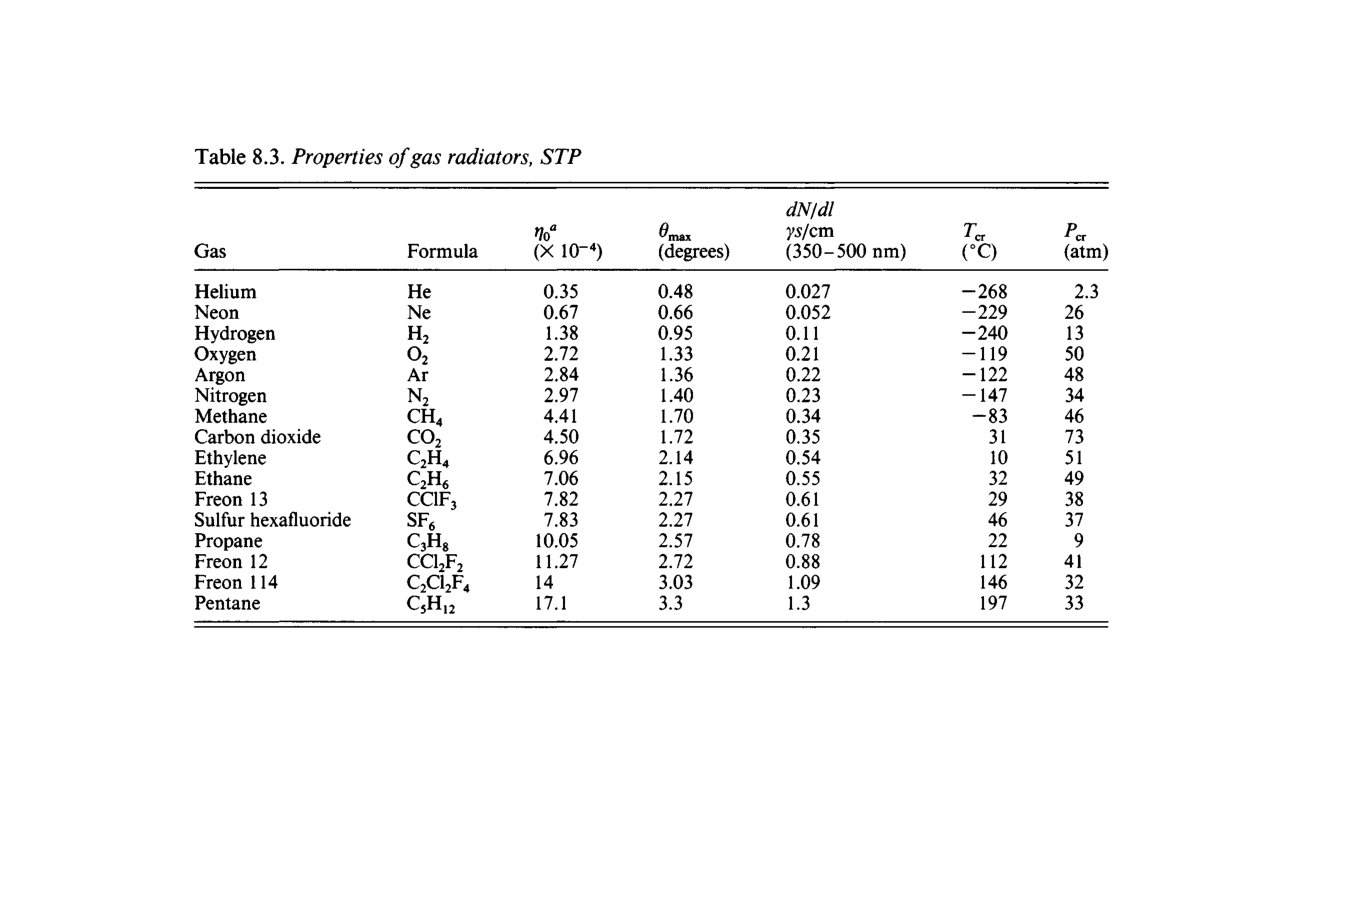
\includegraphics[width=0.8\textwidth, height=0.6\textheight]{./Images/gas_radiators}
  \end{center}
\end{frame}  

\begin{frame}{\textcolor{Goldenrod}{Threshold Cherenkov Counter}}
  \begin{center}
    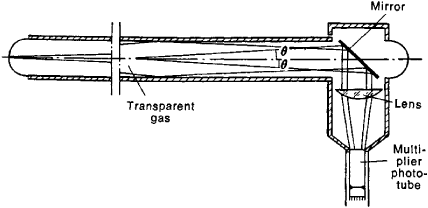
\includegraphics[width=0.7\textwidth, height=0.3\textheight]{./Images/threshold_gas_Cherenkov_detector}
  \end{center}
  The main characteristics of threshold Cherenkov counters
  is the detection efficiency. 

\itt
\item[$\bullet$] \hlt{Magenta}{A threshold Cherenkov counter should
    detect all particles with velocities greater than some threshold
    value.}
\item[$\bullet$] use number of radiated photons to identify particles
  (useful when we don't know the composition of incoming beam)
  \tti
\end{frame}

\begin{frame}{\textcolor{Goldenrod}{Threshold Cherenkov Counter}}
  \hlt{LimeGreen}{Cerenkov light in the material will pass through the exit face
  provided that the Cerenkov angle is smaller than the critical angle.
  Thus, the detected particles satisfy the relation:}
  \[
    \cos^{-1}(1/n\beta) \leq \sin^{-1}(1/n)
  \]
  The counter detects particles over a velocity range $ [1/n,
  1/\sqrt{n^2 -1}]$\\
  The detection efficiency of a threshold counter increases rapidly as the
  velocity of the incident particles.
\end{frame}

\begin{frame}{\textcolor{Goldenrod}{Threshold Cherenkov Counter
      Efficiency}}
  \begin{center}
    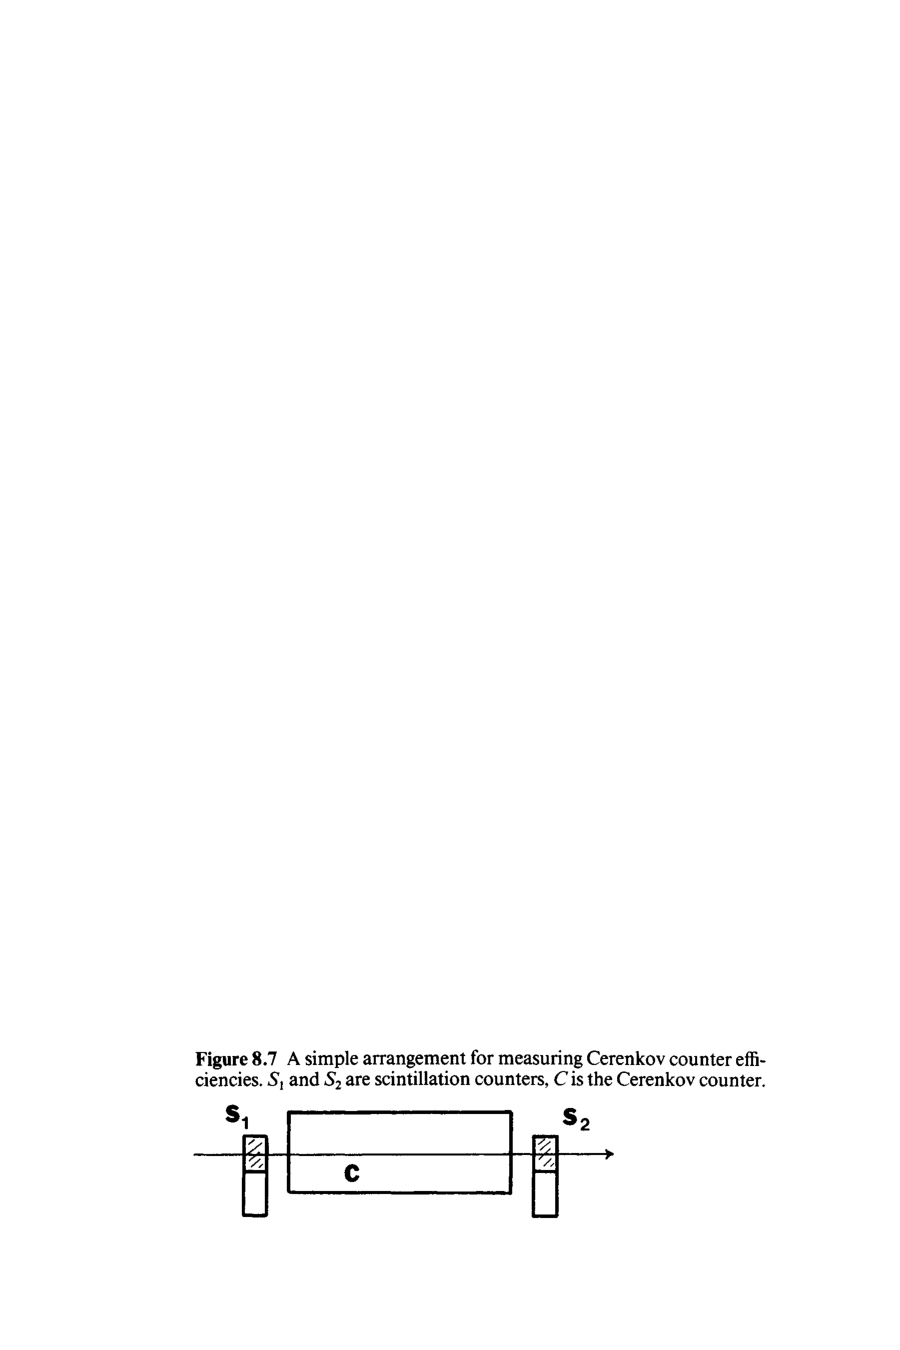
\includegraphics[width=0.8\textwidth,
    height=0.25\textheight]{./Images/threshold_detector_eff}\\
  \end{center}
  The Cerenkov counter efficiency:
  \[
    \epsilon =  \frac{S_1 \otimes S_2 \otimes C} {S_1 \otimes S_2}
  \]
  
  The detection efficiency:
  \[
    \epsilon(\beta) = 1 - p(0, N_e) = 1 - e^{-N_e}
  \]
  {\scriptsize
    Where $p(0, N_e)$ is the probability that no electrons were emitted by
    the photocathode of the PMT if the average number is $N_e$.
    (using Poisson distribution for photoelectron emission).
  }
\end{frame}

\begin{frame}{\textcolor{Goldenrod}{Threshold Cherenkov Counter}}
  \itt
\item[$\Box$] Since $N_e = N_0 L \sin^2\theta$, therefore $\epsilon
  \uparrow L[N_0] $
\item[$\Box$] The shape of the efficiency curve is affected by energy
  loss in the gas, dispersion, and the velocity spread of the incident
  beam.
\item[$\Box$] The threshold velocity resolution of the counter can be
  determined
  \[ N_e = N_0 L (1- \frac{\beta^2_t}{\beta^2}) \to
    \frac{\Delta\beta}{\beta}\approx \frac{N_e}{2(N_0L - N_e)}
  \]
\item[$\Box$] \hlt{Orange}{The behavior of the detection efficiency
    near threshold can be affected by the production of knock on electrons
    (delta rays). It is possible for a massive particle with $\beta <
    \beta_t$ to collide with an electron and knock it out with velocity
    greater than $\beta_t$.}
\item[$\Box$] \hlt{Magenta}{Fortunately, the delta rays are emitted with a
  perpendicular angular distribution}
  \tti
\end{frame}
\begin{frame}{\textcolor{Goldenrod}{Threshold Cherenkov Counter}}
  \begin{center}
  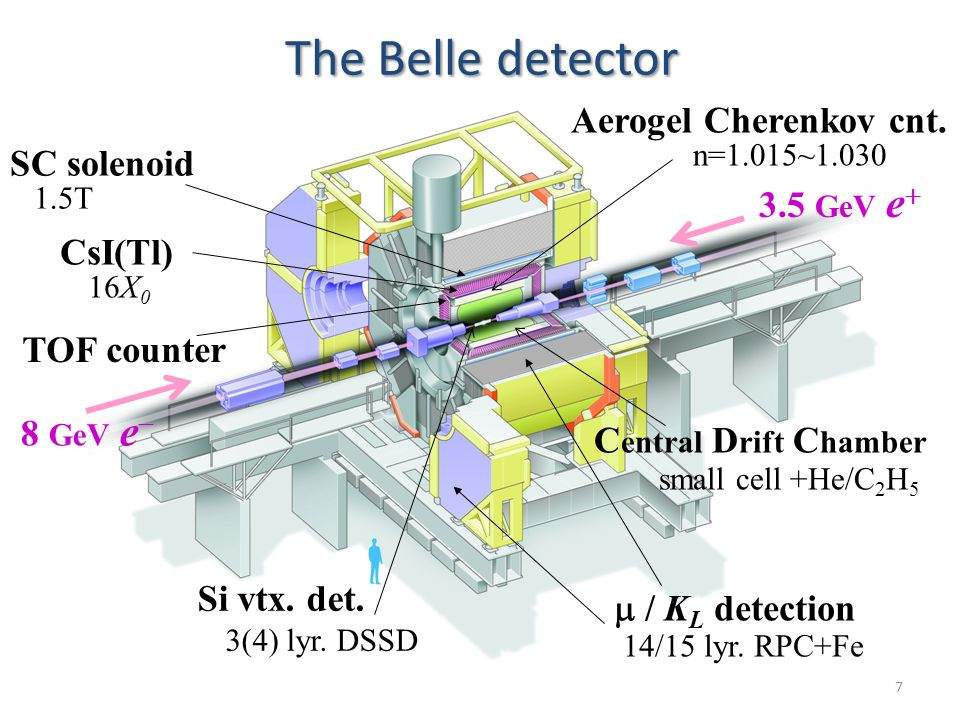
\includegraphics[width=0.7\textwidth,
  height=0.45\textheight]{./Images/Belle_detector_01}\\
  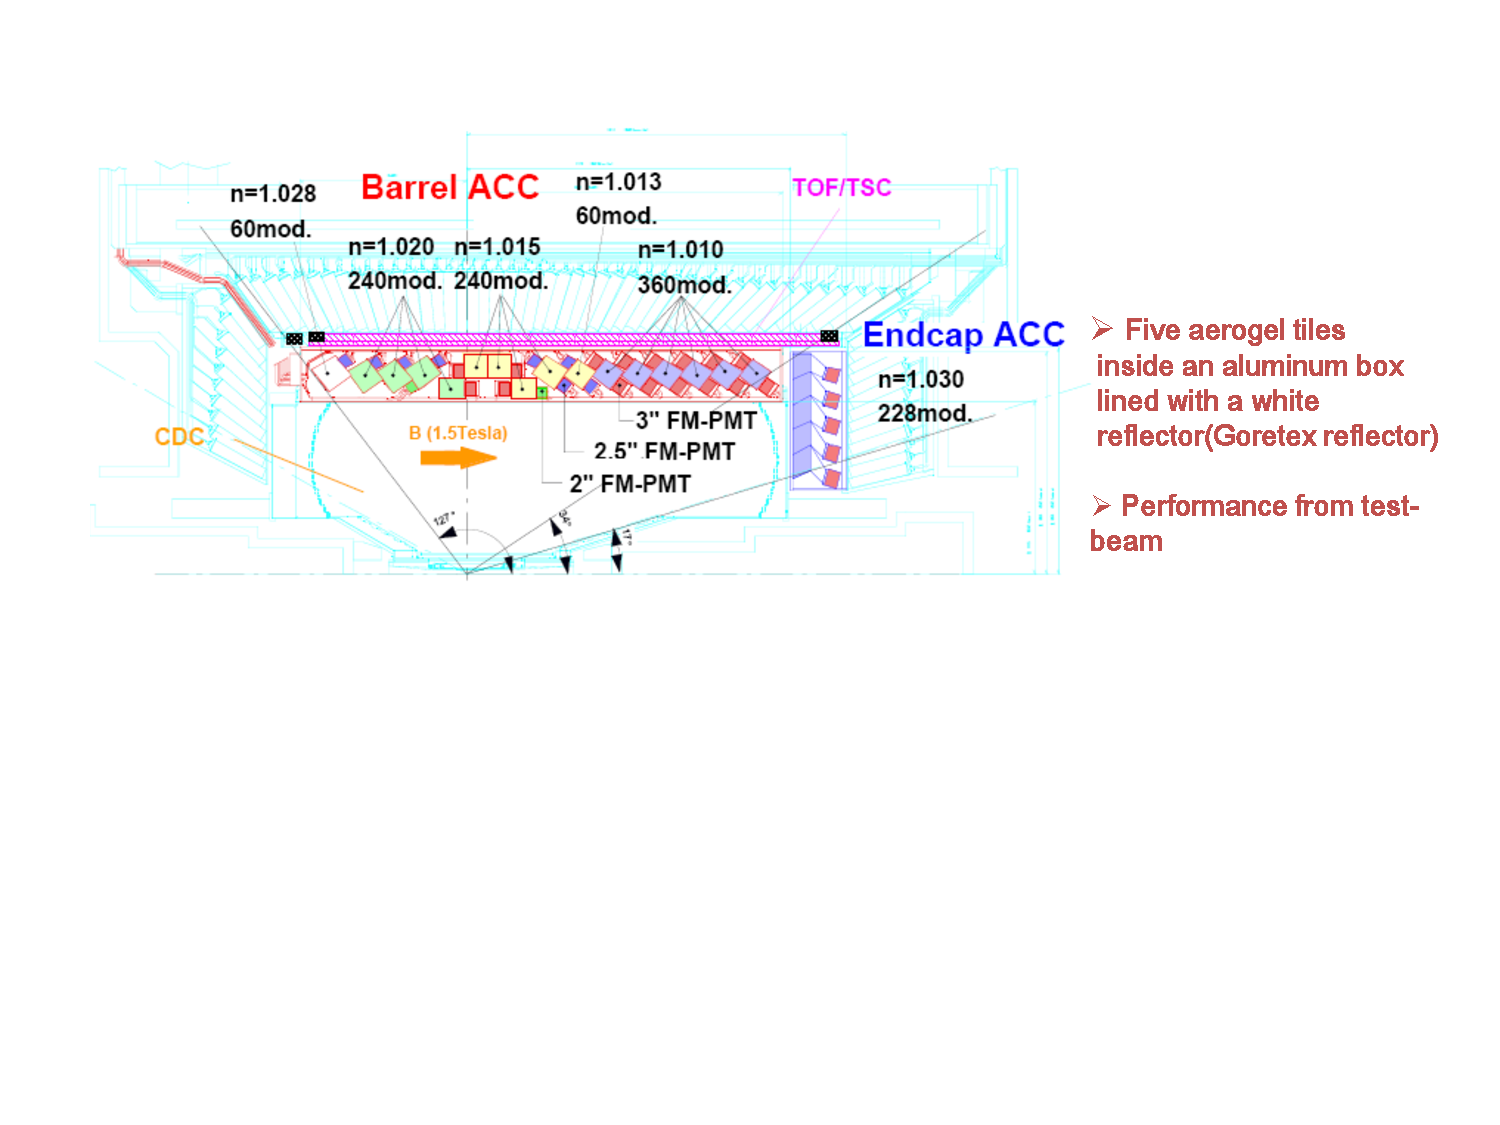
\includegraphics[width=0.7\textwidth,
  height=0.35\textheight]{./Images/Belle_detector_02}\\
  \end{center}
  
  \itt
  \item BELLE experiment: $e^-e^+$ collider  searching for CP violation in
    B-meson decays.
  \tti
\end{frame}

%%%%%%%%% Differential Cherenkov detectors

\begin{frame}{\textcolor{Goldenrod}{Differential Cherenkov Counter}}
  \(
  \<{0.5\textwidth}
  \img{differential_cherenkov_detectors}
  \>
  % differential_cherenkov_detectors_01
  \<{0.65\textwidth}
  \hlt{Blue}{A differential Cerenkov counter can measure the velocity of a particle
    by only accepting Cerenkov light in a small annulus around some angle
    $\theta$.}
  \itt
\item Using such a counter, it is possible to provide a signal for the
  presence of a given mass particle.
\item Cerenkov light in the radiator gas is reflected by a spherical
  mirror. The cones of light appear to the mirror as a ring source at
  infinity. The image consists of a ring in the focal plane of the mirror
  with radius $R = f\tan\theta$
  \tti
  \>
  \)
\end{frame}

\begin{frame}{\textcolor{Goldenrod}{Differential Cherenkov Counter}}
  \hlt{Blue}{A diaphragm containing a slit of width $\Delta r$  placed in front of the PMTs
  will only accept light from within the angular range}
  \[
    \Delta \theta =
    \cos^2\theta \frac{\Delta r}{f} \to \frac{\Delta \beta}{\beta} = \tan\beta\Delta\theta
  \]
  \itt
\item \hlt{Red}{The minimum obtainable angular resolution is mainly limited by
  dispersion.}
  $\Delta \theta_{disp} =  \frac{\Delta n}{n \tan\theta}$
  
\item \hlt{Magenta}{The angular resolution is also affected by beam divergence, optical
  aberrations, multiple scattering in the radiator, energy loss in the
  radiator, and diffraction}
  \tti  
\end{frame}

\begin{frame}{\textcolor{Goldenrod}{Differential Cherenkov Counter}}
  \(
  \<{0.45\textwidth}
  \img{differential_cherenkov_detectors_02}
  \>
  \<{0.45\textwidth}
  \img{differential_cherenkov_detectors_03}
  \>
  \)
  \hlt{LimeGreen}{differential gas counter (DISC) used in a hyperon beam at CERN. This
    counter uses an adjustable optical system to correct for dispersion
    and geometric aberrations. A velocity resolution $\Delta \beta \sim
    5\times 10^{-5}$}
\end{frame}

\begin{frame}{\textcolor{Goldenrod}{Ring Imaging Cherenkov Counter}}
  \(
  \<{0.7\textwidth}
  \hlt{Red}{The DISC counter is only suitable for use in a well-collimated beam of
  particles.}

\itt
\item[$\bullet$] \hlt{JungleGreen}{We can use the Cerenkov effect to
    measure the velocities of secondary particles arising from an
    interaction alongside with an independent measurement of the momenta
    to identify the particles masses.}
  
\item[$\bullet$] \hlt{NavyBlue}{Ring Imaging Cerenkov (RICH):
    The radiating medium is contained
    between two spheres surrounding the target or intersection point. The
    Cerenkov light reflects off the mirror and is focused onto a ring at
    the detector surface.}
  \tti
  \>
  \<{0.55\textwidth}
  \img{RICH_counters_02}
  \>
  \)
\end{frame} 

% \begin{frame}{\textcolor{Goldenrod}{Ring Imaging Cherenkov Counter}}
%   \small 
%   \itt
% \item \alert{Measure both $\theta_C $ and $N_e$}
% \item \alert{Very useful for particle identification over large surfaces}
% \item \alert{Requires photodetectors with single photon detection capability}
% \item With this geometry the radius of the ring is directly related to
%   the Cerenkov angle through $ r = f\tan\beta$
% \item \hlt{Blue}{Resolution:} $\frac{\Delta \gamma}{\gamma} =
%   \frac{n\gamma^2\beta^3}{\sqrt{N_0 L}} \frac{2\Delta r}{R}$. $R$ is the
%   radius of curvature of the mirror, and $\Delta r$ is the uncertainty
%   in the ring radius at the detector plane due to all sources.
% \item Since the number of photons expected per particle is very small,
%   most RICH designs have concentrated on collecting
%   photons from the ultraviolet portion of the spectrum. ( larger
%   $N_\gamma$, UV $\gamma \to photoelectrons\, 100\% \,efficiency$ )
% \item \hlt{Magenta}{The Cerenkov radiating gas must be transparent in the
%   ultraviolet. This restricts the radiator to a few gases, including the
%   noble gases and nitrogen}
%   \tti
% \end{frame} 

\begin{frame}{\textcolor{Goldenrod}{Ring Imaging Cherenkov Counter}}
  \hlt{Orange}{The radiator fills the volume between the spherical surfaces with
    radii $R_S$ and $R_D$. In general, one takes $R_D = R_S/2$, since the focal
    length $f$ of a spherical mirror is $R_S/2$.}
\itt
\item Because all Cherenkov photons
  are emitted at the same angle $\theta_c$ with respect to the particle
  trajectory pointing away from the sphere centre, all of them will be
  focused to the thin detector ring on the inner sphere. One can
  easily calculate the radius of the Cherenkov ring on the detector
  surface
  \[
    r  = f \theta_C = \frac{R_S}{2} \theta_C \to \beta = \frac{1}{\cos(2r/R_s)} 
  \]
\item  If the momentum of the charged particle is known, then
  we can get it's mass from
  \[
    p  = \frac{m_0 c \beta}{\sqrt{1 - \beta^2}}
  \]
\item 
  \tti
\end{frame} 

\begin{frame}{\textcolor{Goldenrod}{Ring Imaging Cherenkov Counter}}
  \(
  \<{0.4\textwidth}
  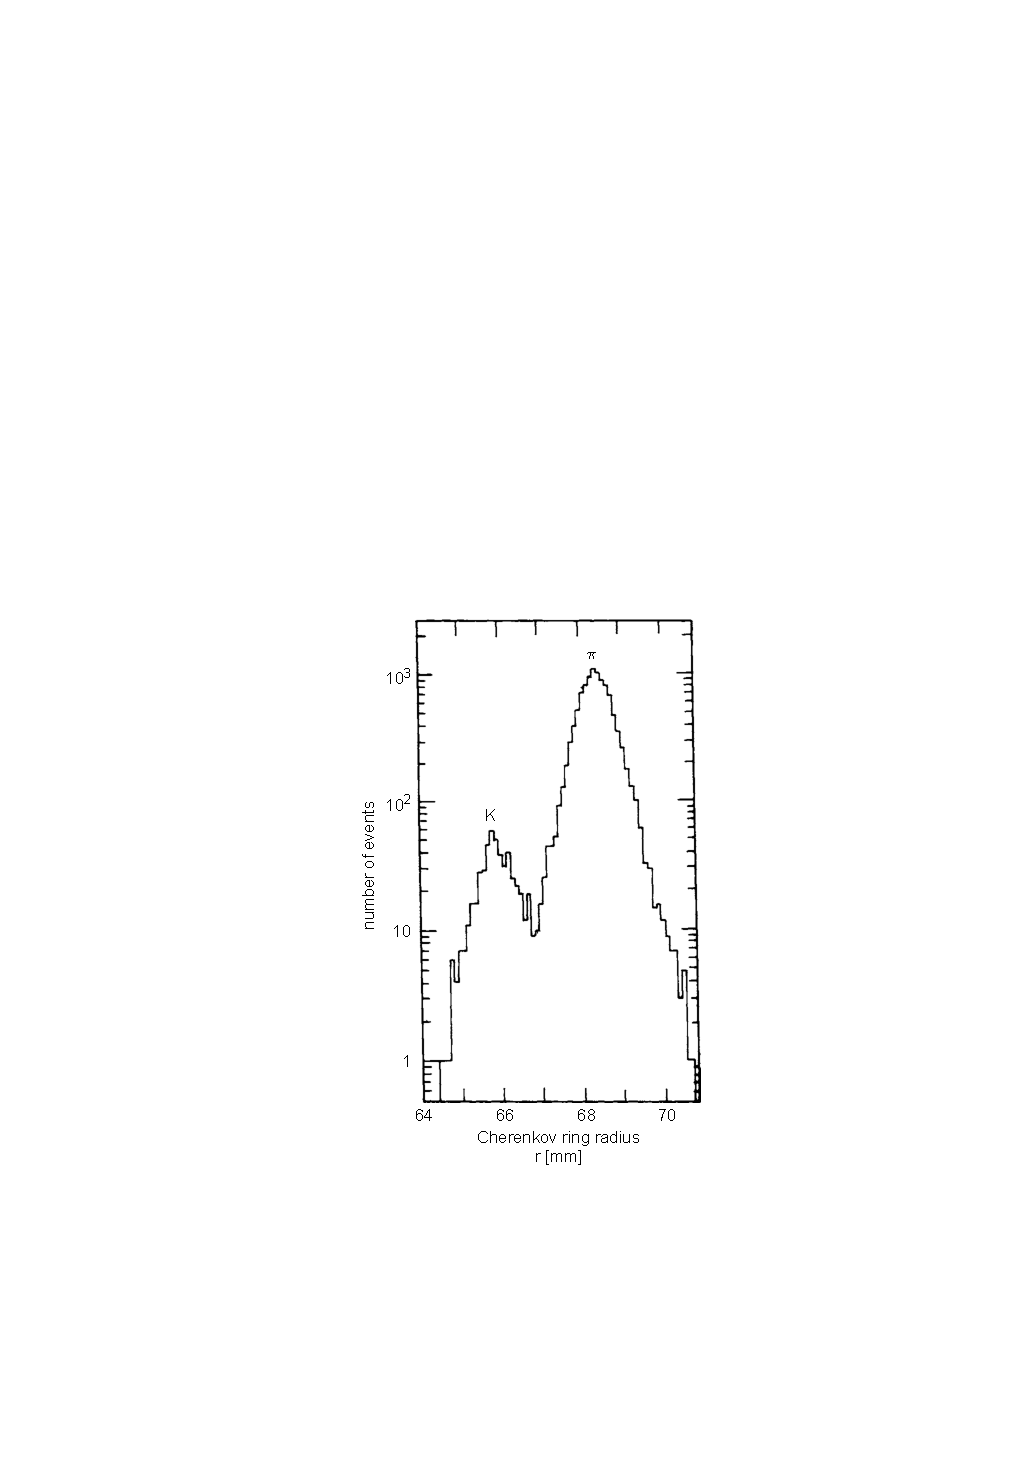
\includegraphics[width=0.99\textwidth, height=0.85\textwidth]{./Images/RICH_counters_03}
  \>
  \<{0.75\textwidth}
  \itt
\item \hlt{Magenta}{The most crucial aspect of RICH counters is the detection of
  Cherenkov photons with high efficiency on the large detector
  surface.}
  (Multiwire proportional chambers are good choices for measuring $\gamma$ coordinates).
  % Since
  % one is not only interested in detecting photons, but also in measuring
  % their coordinates, a position-sensitive detector is necessary.
\item Distribution of Cherenkov ring radii in a pion-kaon beam at  
  $200 GeV/c$. The Cherenkov photons have been detected in a multiwire pro-
  portional chamber filled with helium $(83\%)$, methane $(14\%)$ and
  TEA (triethylamine) $(3\%)$.
\item \alert{Better Cherenkov rings are obtained from fast heavy ions, because the
    number of produced photons is proportional to the square of the
    projectile charge.}
  \tti
  \>
  \)
\end{frame} 
\begin{frame}{\textcolor{Goldenrod}{Ring Imaging Cherenkov Counter: LHCb}}
  \begin{center}
    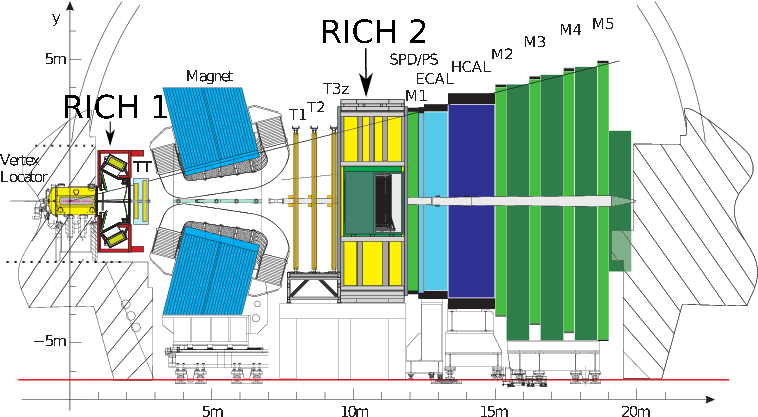
\includegraphics[width=0.8\textwidth, height=0.4\textheight]{./Images/RICH_counters_04}\\
  \end{center}
\small
  \itt
\item[$\bullet$] The Ring-
  Imaging Cherenkov (RICH) system is one of the key components of LHCb.
\item[$\bullet$] This provides charged particle identification ($\pi
  , K , p$)over
  a wide momentum range, from $2-100 GeV/c$.
\item[$\bullet$] It consists of two RICH detectors that cover between them the
  angular acceptance of the experiment, $15 - 300 mrad$ with respect to
  the beam axis.
  \tti
\end{frame}  

\begin{frame}{\textcolor{Goldenrod}{Ring Imaging Cherenkov Counter:LHCb}}
  \begin{center}
    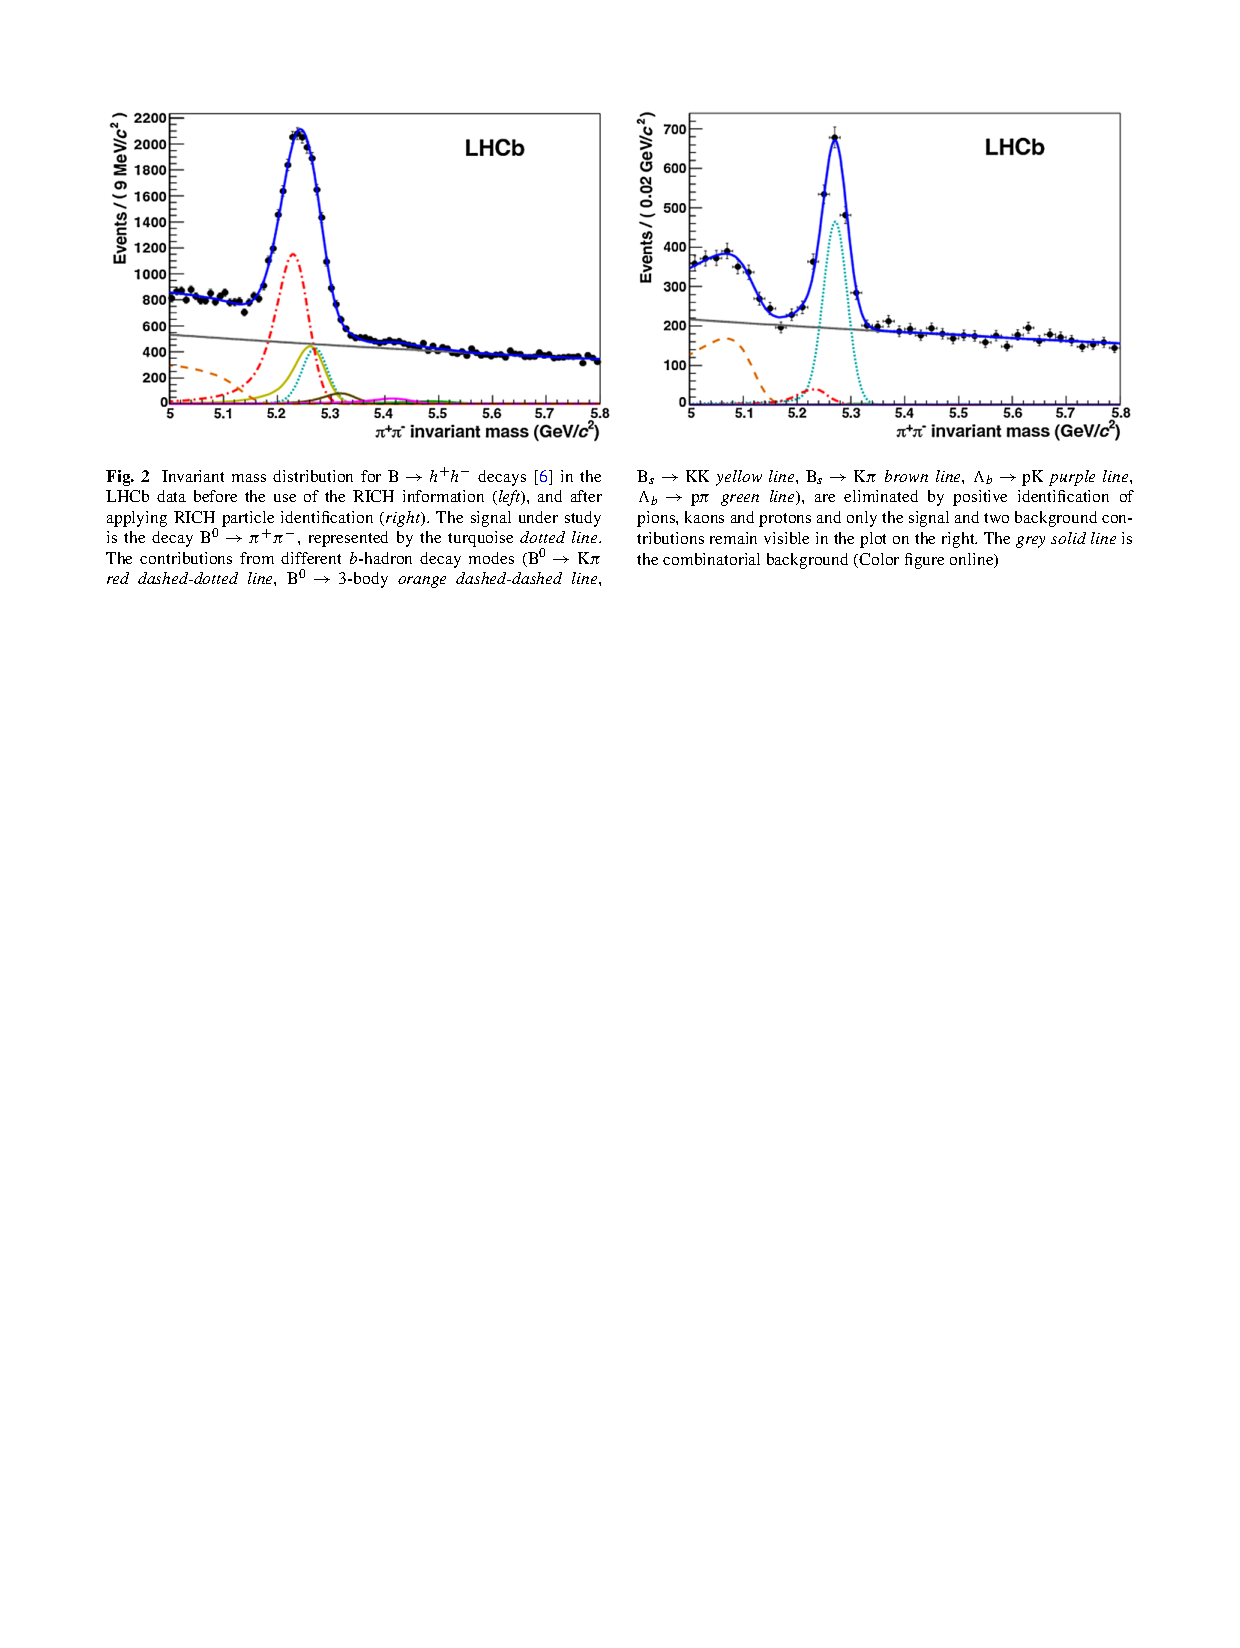
\includegraphics[width=0.95\textwidth,height=0.6\textheight]{./Images/RICH_counters_05}
  \end{center}
\end{frame}  

%%%%%%%% TRD , TRT
\begin{frame}{\textcolor{Goldenrod}{Transition Radiation }}

  \hlt{Blue}{Transition Radiation (TR) happens when a charged particle moves through
    an inhomogeneous media (different dielectric constants)}
  
  \itt
\item The energy spectrum radiated by a charged particle with a Lorentz factor
  $\gamma$ traversing an interface between two dielectric media (with
  dielectric constants $\epsilon_1$ and $\epsilon_2$) is as following:
  \[
    \frac{dE}{d\nu d\Omega} =  \frac{\alpha^2}{\pi^2}
    (\frac{\theta}{\gamma^{-2}+\theta^2 +(1-\epsilon^2_1)} + \frac{\theta}{\gamma^{-2}+\theta^2 +(1-\epsilon^2_2)})^2
  \]
\item Since TR depends on $\gamma$, for a wide
  momentum range $(1-100 GeV/c)$ where $e^+/e^-$ are the
  only particles producing transition radiation. Kaons can also be
  separated from pions on the basis of TR in a certain momentum range
  (roughly $200 - 700 GeV/c$).
  \tti
\end{frame}  
\begin{frame}{\textcolor{Goldenrod}{Transition Radiation: in a Single
    Foil}}
\(
\<{0.4\textwidth}
\img{TRD_10}
\>
\<{0.68\textwidth}
\hlt{Blue}{A single foil has two interfaces to the surrounding medium at which
the index of refraction changes. Therefore, one needs to sum up the
contributions from both interfaces of the foil to the surrounding
medium:}
\[
  \frac{dE}{d\nu d\Omega} |_{foil} = \frac{dE}{d\nu d\Omega}
  |_{interface} \times 4\pi \sin\theta_1/2
\]

\alert{Since the emission probability for a TR photon in the plateau region is of
  order $\alpha/\pi$ per interface. For this to lead to a significant particle
  discrimination one needs to realize many of theses interfaces in a
  single radiator.}
\>
\)  
\end{frame}
\begin{frame}{\textcolor{Goldenrod}{Transition Radiation: Spectrum}}
\(
\<{0.65\textwidth}
\hlt{LimeGreen}{TR production as a function of: the Lorentz factor $\gamma$ (upper panel,
  corresponding to an electron momentum of $0.2, 0.5, 1 and 2 GeV/c$),
  foil thickness $l_1$ (middle panel) and foil spacing $l_2$ (lower
  panel).}
\itt
\item TR is very useful in the X-ray range, which is why Xe detectors are
  popular
\item \alert{While Cerenkovs discriminate on beta, TRDs are sensitive to
    gamma, so they are complementary}
  \tti
  \>
\<{0.45\textwidth}
\img{TRD_11}
\>
\)  
\end{frame}

\begin{frame}{\textcolor{Goldenrod}{Transition-Radiation Detectors}}
  \(
  \<{0.4\textwidth}
  \img{TRD_12}
  \>
  \<{0.65\textwidth}
  \itt
\item Due to the very small TR emission angle, the TR signal generated in a
  detector is overlapping with the ionization due to the specific energy
  loss $dE/dx$ and a knowledge (and proper simulation) of $dE/dx$.
\item due to the large tails in the energy loss spectrum for pions,
  the detector has to have many layers. In case the full charge signal
  is available the discrimination is done using either a normal mean,
  a truncated mean.
\item \hlt{Red}{There are two main types of TRDs: differential like ATLAS, and
  total energy measurement like Hermes}
  \tti
  \> 
  \)  
\end{frame}

\begin{frame}{\textcolor{Goldenrod}{Transition-Radiation Detectors}}
  \begin{center}
    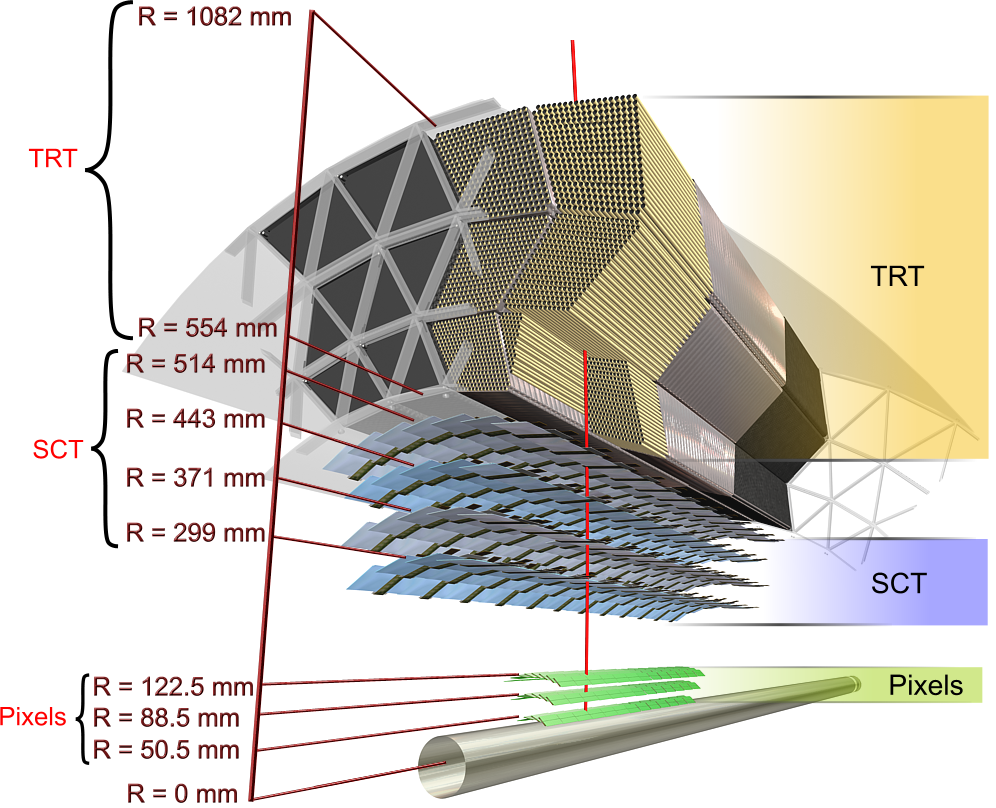
\includegraphics[width=0.6\textwidth, height=0.4\textheight]{./Images/TRD_01}
  \end{center}
\scriptsize
  \itt
\item[$\bullet$] \alert{The ATLAS transition-radiation tracker (TRT) is the
  largest present-day TRD detector.}
\item[$\bullet$] The TRT is part of the ATLAS inner detector and it
  is used both for charged-particle tracking and electron/pion
  separation. It consists of $370 000$ cylindrical drift tubes (straws).
  Made from kapton and covered by a conductive film, the straw tube
  serves as cathode of a cylindrical proportional drift counter.
\item[$\bullet$] A central $30 \mu m$-diameter gold-plated tungsten
  wire serves as anode. The layers of straws are interleaved with
  polypropylene foils or fibres working as radiator. The tubes are
  filled with a gas mixture.
  \tti
\end{frame}  

\begin{frame}{\textcolor{Goldenrod}{Transition-Radiation Detectors}}
  \(
  \<{0.4\textwidth}
  \img{TRD_02}
  \>
  \<{0.7\textwidth}
  \small
  A simiulated $ B^0_d \to J/\psi (\to e^+e^-) K_s(\pi^+\pi^-)$
  \itt
% \item The coordinate determination is performed by a drift-time measure-
%   ment resulting in a spatial resolution of about $130 \mu m$.
\item The
  electron/pion separation is based on the energy deposition.
\item A typical
  energy of the transition-radiation photon in the TRT is $8 -10keV$, while
  a minimum-ionising particle deposits in one straw about $2keV$ on
  average
\item \textcolor{green}{As separation parameter the number of
  straws along the particle track having an energy deposition exceeding
  a certain threshold can be defined.}
  \tti
  \>
  \)
\end{frame}  


\begin{frame}{\textcolor{Goldenrod}{Transition-Radiation Detectors}}
  \begin{center}
    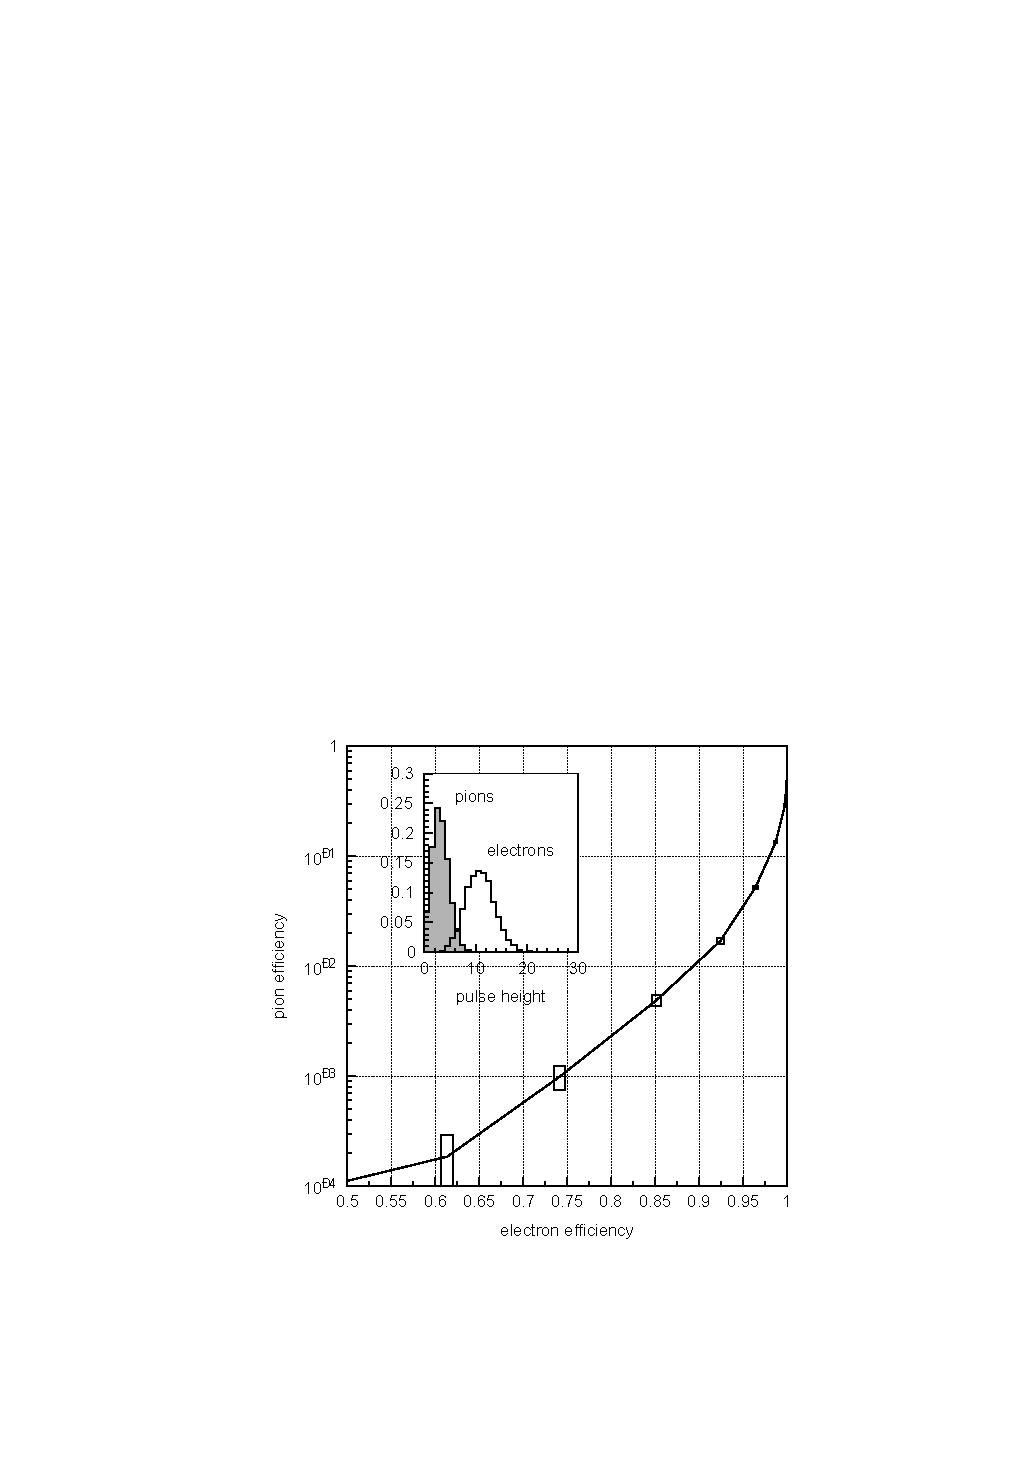
\includegraphics[width=0.6\textwidth, height=0.4\textheight]{./Images/TRD_03}
  \end{center}
  \textcolor{Orange}{Electron/pion separation capability measured with a prototype.
    The insert shows the energy depositions in a single straw for pions
    and electrons.}
\end{frame}  


%%%%%%%%%%%%%% APPENDIX
% All your regular slides
% After your last numbered slide

% \appendix
% \newcounter{finalframe}
% \setcounter{finalframe}{\value{framenumber}}
% \beginbackup
% \begin{frame}[noframenumbering]
% \hlt{ForestGreen}{Additional material}
% \end{frame}

% \backupend
\end{document}
